\section{Versuchsaufbau und Inbetriebnahme} \label{sec:versuchsaufbau}

Bevor das Roboterfahrzeug (im Folgenden bezeichnet mit \glqq Jetbot\grqq{}) programmiert und getestet werden kann auf seine Fähigkeiten sich autonom mittels CNN und Transfer Learning fortzubewegen und dabei jegliche Kollisionen zu vermeiden, muss dieses zunächst gebaut und in Betrieb genommen werden. Dieser Abschnitt wird einen kurzen Überblick über die verwendete Hardware geben und kurz beschreiben, wie der Jetbot zum Programmieren aufgesetzt wird. 

\subsection{Benötigte Komponenten}

\autoref{tab:Tabelle3.1} zeigt eine Liste aller benötigten Komponenten und Materialien für den Roboter. Von besonderer Wichtigkeit für die Anwendung Neuronaler Netze in diesem Versuch ist zum einen das Gehirn des Jetbot, der \textbf{Jetson Nano Mikrocontroller} von Nvidia. Dabei handelt es sich konkret um einen auf ARM basierenden Computer, der dafür entwickelt wurde mittels seiner integrierten GPU (Graphical Processing Unit) mehrere neuronale Netze parallel zu berechnen. Er ist ausgestattet mit einer Quad-core ARM Cortex-A57 MPCore CPU, einer NVIDIA Maxwell GPU mit 128 CUDA cores und GB 64-bit LPDDR4, 1600MHz 25.6 GB/s RAM. Die zweite wichtige Komponente ist die Kamera des Roboters. Dabei handelt es sich um eine 8MP \textbf{$160^\circ$ FOV Kamera} mit IMX219 Sensor und 3280x2464 Pixeln Auflösung, welche für Gesichtserkennung, Objektklassifizierung, und Echtzeitmonitoring entwickelt wurde.

\begin{figure}[H]
    \begin{subfigure}{0.5\textwidth}
        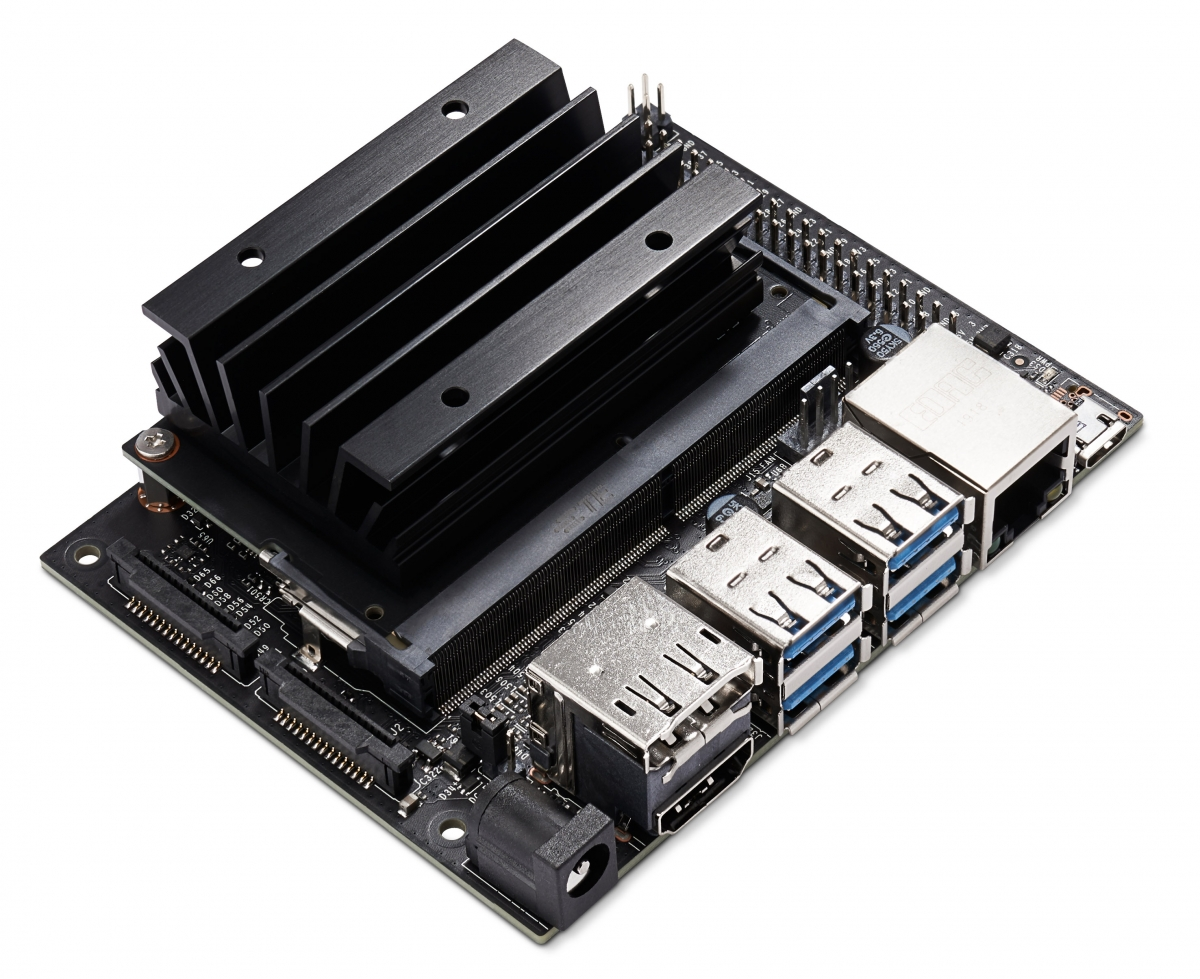
\includegraphics[width=0.9\linewidth]{Bilder/jetson-nano.jpg}
    \end{subfigure}
    \begin{subfigure}{0.5\textwidth}
        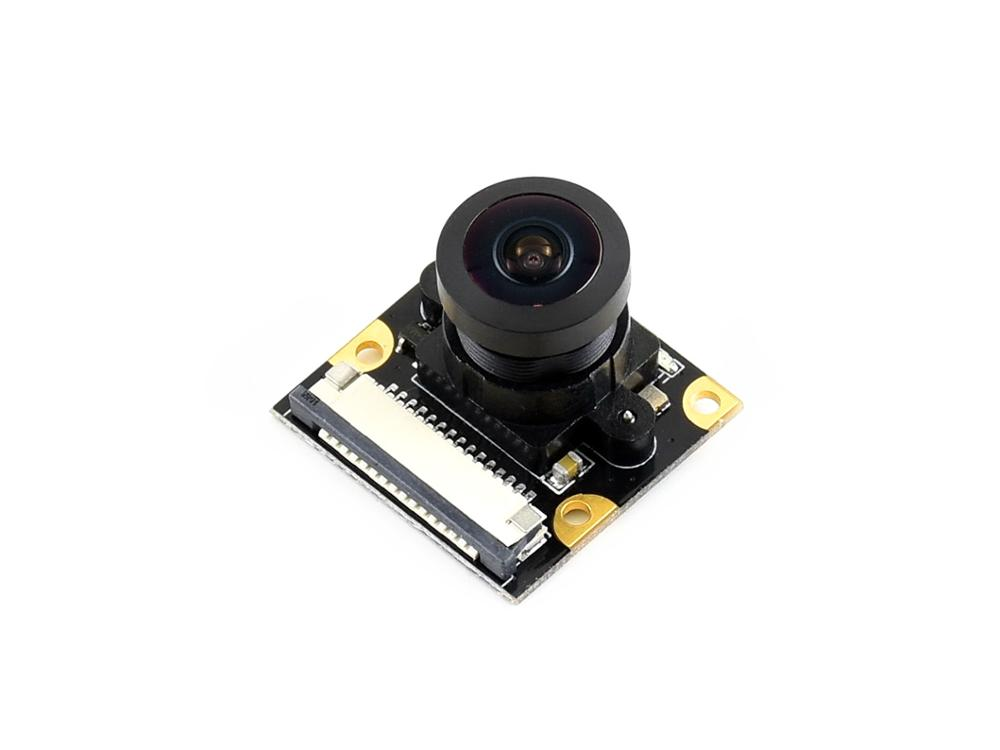
\includegraphics[width=0.9\linewidth]{Bilder/kamera.jpg}
    \end{subfigure}
    \label{fig:Bild3.1}
    \caption[Jetson Nano und Weitwinkelkamera]{Jetson Nano Mikrocontroller und $160^\circ$ Weitwinkelkamera}
\end{figure}

\begin{table}[H]
    \footnotesize
    \begin{longtable}[c]{|l|l|l|l|}
    	\hline
    	\textbf{Nr.} & \textbf{Bauteil}   & \textbf{Anzahl} & \textbf{Bemerkung}                \\ \hline
    	\endfirsthead
    	%
    	\endhead
    	%
    	1            & Jetson Nano        & 1               & 4\,GB RAM Variante                \\
    	2            & Mikro SD Karte     & 1               & mind. 64\,GB                      \\
    	3            & Karosserie         & 1               & ---                               \\
    	4            & Kamera-Befestigung & 1               & ---                               \\
    	5            & Abstandshalter für Kamera aus Acryl & 1 & ---                            \\
        6            & Kamera             & 1               & IMX219-160 Weitwinkel             \\
        7            & WLAN-Stick         & 1               & RTL8121 Chipsatz                  \\
        8            & Erweiterungsboard  & 1               & für Jetson Nano                   \\
        9            & Motor              & 2               & \glqq TT\grqq-Bauform             \\
        10           & Rad                & 2               & 60mm Durchmesser                  \\
        11           & Kugelrolle         & 2               & 1'' Durchmesser                   \\
        12           & Steckeradapter EU  & 1               & ---                               \\
    	13           & Ladegerät          & 1               & 12.6 V                            \\
    	14           & Gamepad            & 1               & kabellos                          \\
    	15           & Montagewerkzeug    & 2               & Schraubenzieher                   \\
    	16           & 6-Pin Kabel        & 1               & 9 cm                              \\
    	17           & Schrauben          & 38              & M2 und M3 Gewinde                 \\
    	18           & Lüfter             & 1               & Bauform 4010                      \\
    	19           & SD-Kartenlesegerät & 1               & ---                               \\ \hline
    	\caption[Materialliste]{Auflistung der benötigten Bauteile für den Aufbau des Jetbot}
    	\label{tab:Tabelle3.1}
    \end{longtable}
\end{table}

\begin{figure}[H]
    \centering
    \fbox{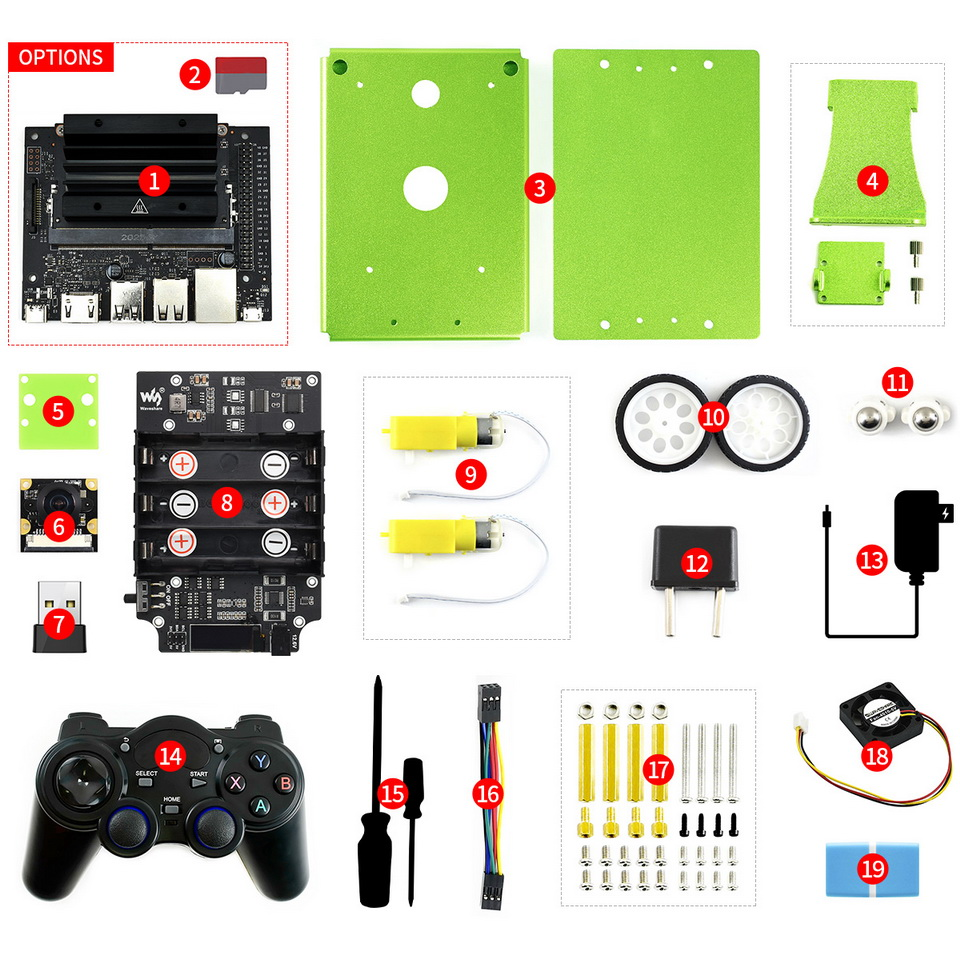
\includegraphics[width=0.53\textwidth]{Bilder/komponenten.jpg}}
    \caption[Komponenten Jetbot]{Darstellung aller verwendeten Komponenten für die Montage des Jetbots}
    \label{fig:Bild3.2}
\end{figure}

\subsection{Hardware-Setup}

Zunächst werden die Motoren auf der Grundfläche des Gehäuses verschraubt. Dieses kann nachfolgen geschlossen werden mit den restlichen Karosserieteilen. Es bietet sich an im nächsten schritt die Räder und Kugelrollen zu montieren, so dass das Gefährt aufrecht stehen kann. Darauf werden die Akkus in dem Erweiterungsboard installiert sowie Abstandshalter an den Ecken angebracht. Das Erweiterungsboard kann dann auf der Karosserie angebracht werden mit vier M2 Schrauben. Auf den im vorherigen Schritt montierten Abstandshaltern wird der Jetson Nano Controller befestigt. Über das 6-Pin Kabel wird anschließend das Erweiterungsboard mit dem Jetson Nano verbunden. Im Anschluss wird der Lüfter auf dem Kühlkörper angebracht und das Lüfterkabel in den PWM-Anschluss gesteckt. Im letzten Schritt wird die Kamerabefestigung am Gehäuse angebracht, der Abstandshalter aus Acryl an an dieser angeschraubt und Abschließend die Kamera montiert. \autoref{fig:Bild3.3} zeigt den fertigen Aufbau des Jetbot Roboterfahrzeugs.

\begin{figure}[H]
    \centering
    \fbox{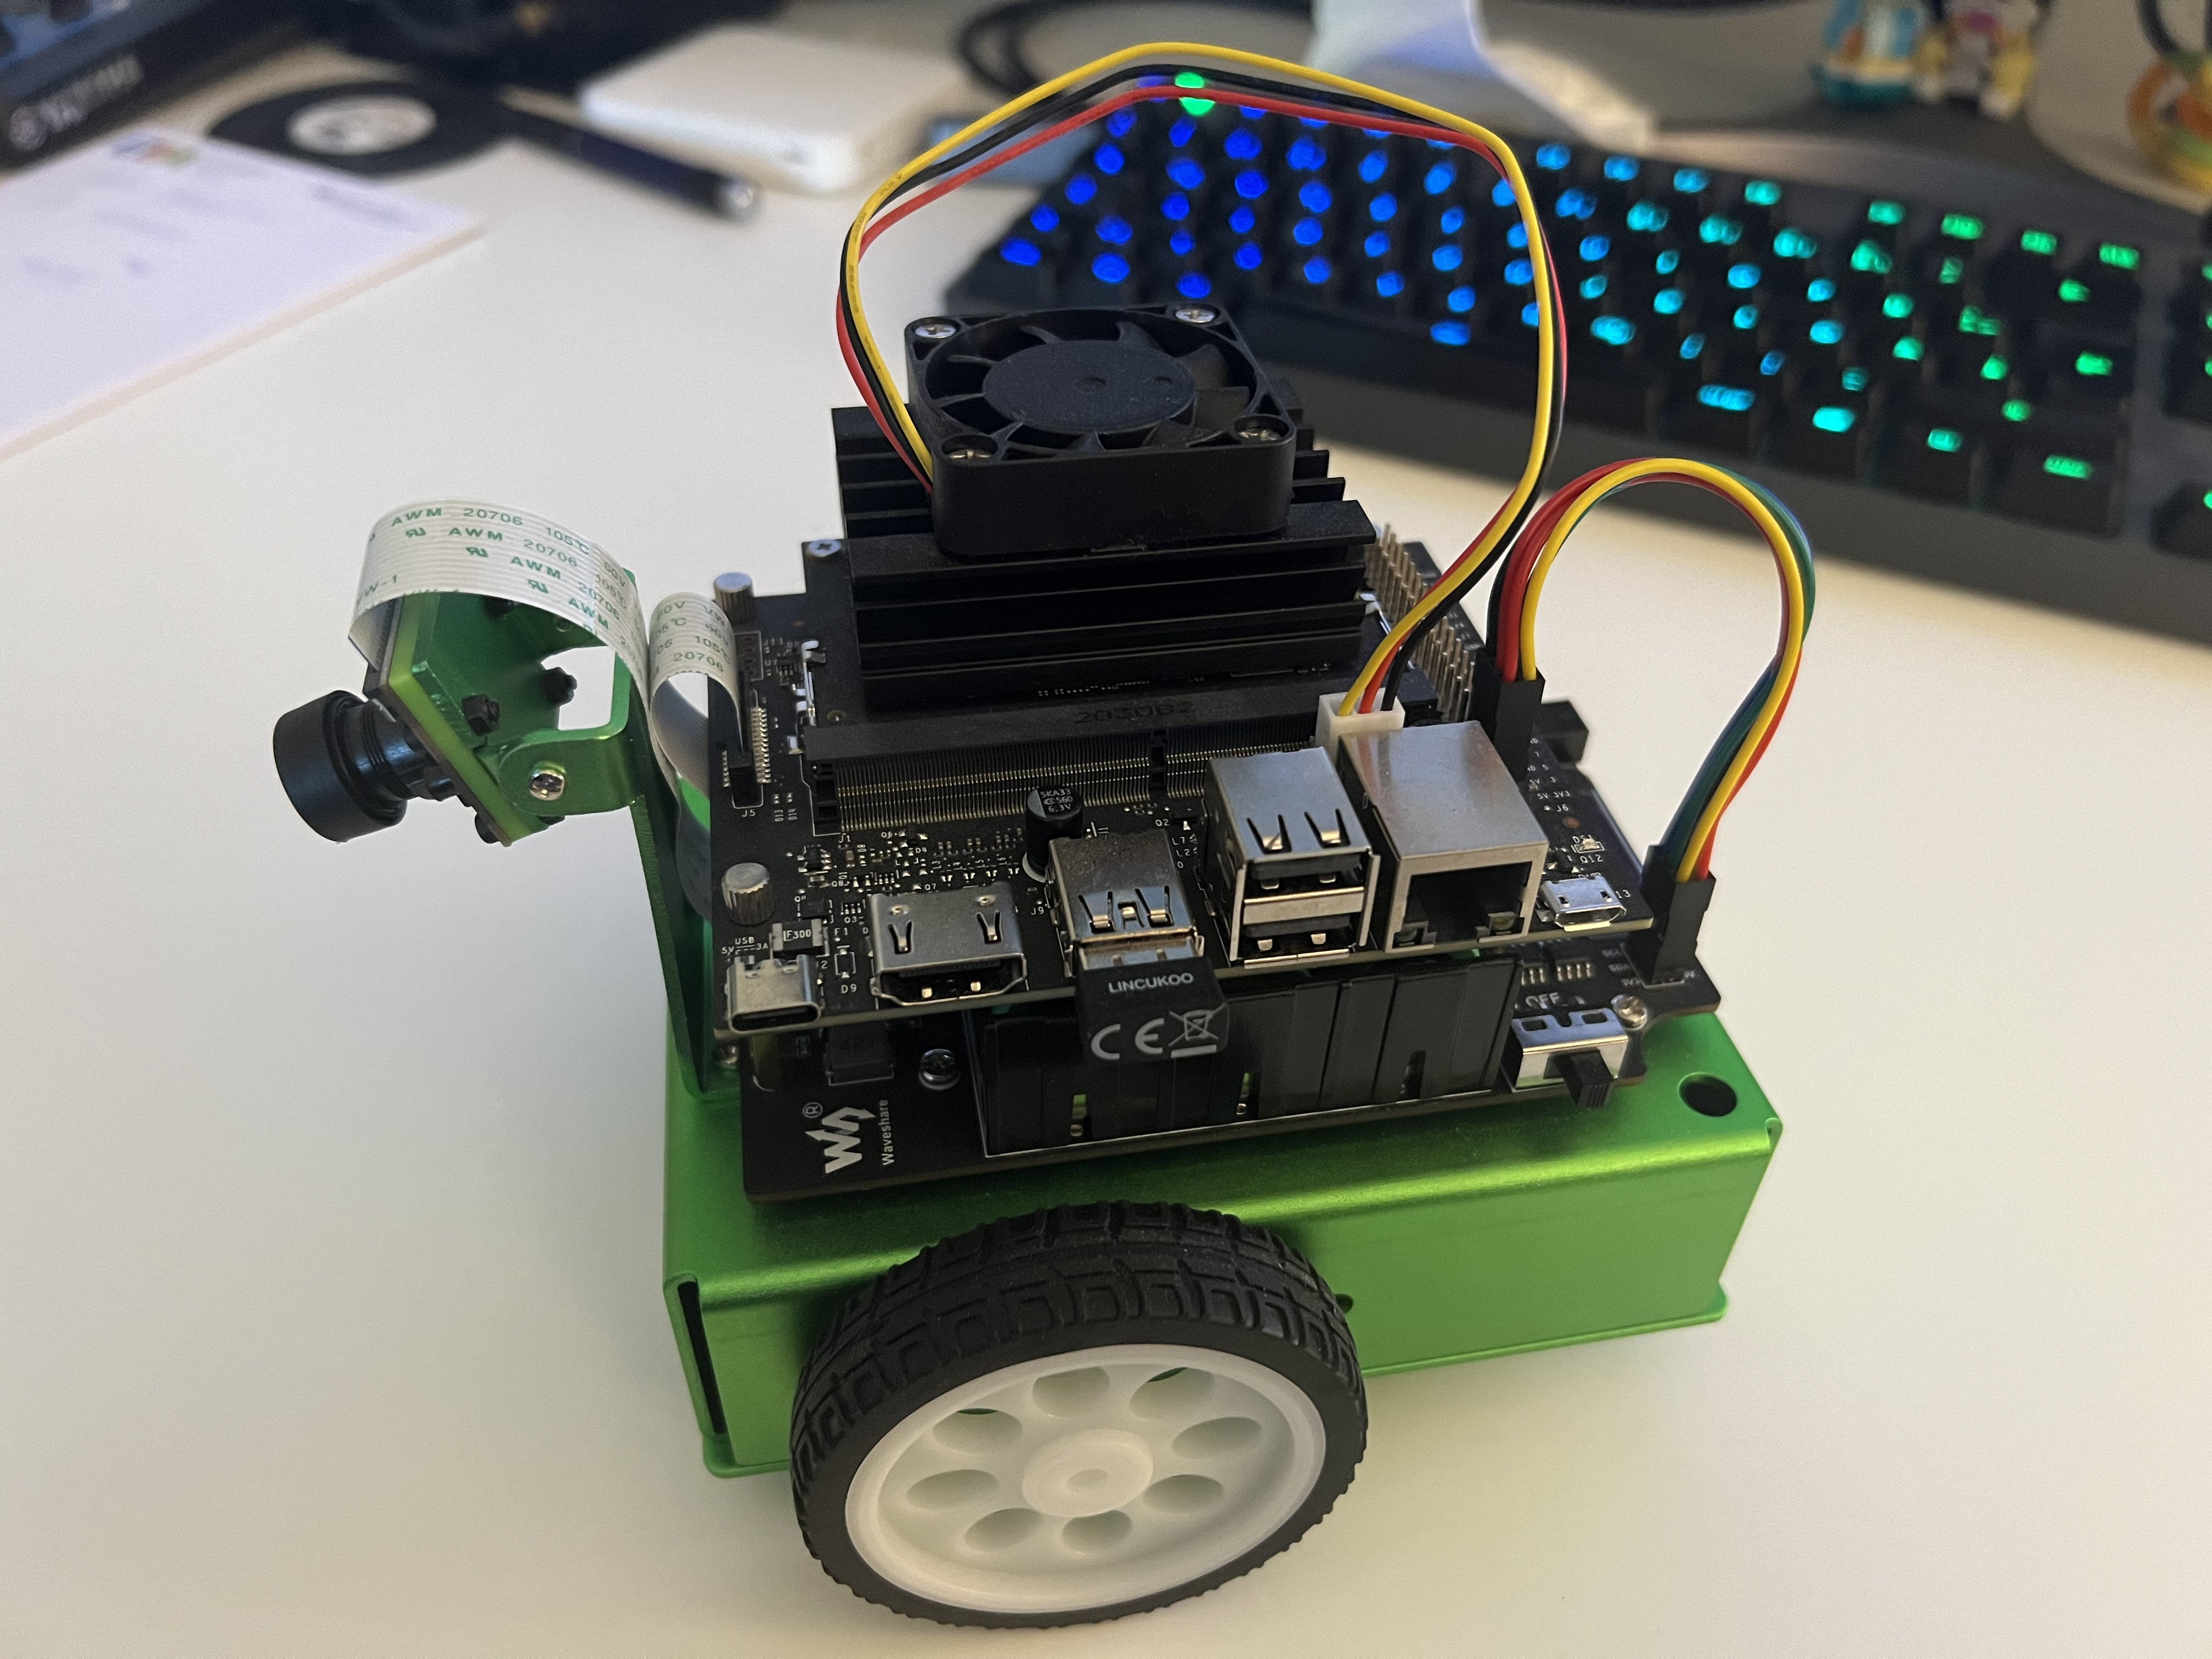
\includegraphics[width=0.98\textwidth]{Bilder/jetbot-aufbau.jpg}}
    \caption[Aufbau Jetbot]{Aufbau des Jetbot-Roboterfahrzeugs}
    \label{fig:Bild3.3}
\end{figure}

\subsection{Software-Setup}

Der erste Schritt ist es sich ein von Nvidia für den Jetson Nano bereitgestelltes Image auf die SD-Karte herunterzuladen. Dieses beinhaltet Ubuntu Linux als Betriebssystem, sämtliche notwendigen Treiber für die Betriebsmittel wie \zB die Kamera und besitzt bereits eine Installation für Python inklusive Jupyter und PyTorch. Worum es sich dabei handelt wird in \autoref{sec:durchführung} geklärt.\\
Die folgenden Schritte sind notwendig, um das Image auf die SD-Karte zu spielen:

\begin{enumerate}
    \item SD-Karte über Lesegerät an beliebigen PC anschließen.
    \item Mit Etcher das heruntergeladene Image auswählen und auf die SD-Karte übertragen.
    \item SD-Karte in den Jetson Nano einstecken.
\end{enumerate}

Der nächste Schritt kann abweichen je nach gewählter Methode. Grundsätzlich ist das Ziel den Jetson Nano mit einem WLAN-Netzwerk zu verbinden. Dazu kann entweder ein Monitor an den HDMI-Port, sowie Maus und Tastatur per USB angeschlossen werden. Nach dem Booten des Systems ist es dann möglich über die Netzwerkeinstellungen eine Verbindung zum WLAN herzustellen. Alternativ ist es möglich über \zB Putty unter Windows oder über das Terminal in Linux oder MACOS auf den Jetson Nano zuzugreifen. Anschließend wird die Verbindung hergestellt über das Kommando\\

\texttt{sudo nmcli device wifi connect <SSID> password <PASSWORD>}. \\

Der Mikrocontroller verbindet sich nun nach dem Einschalten automatisch mit dem ausgewählten Netzwerk. Nachfolgend kann der Jetbot über den Browser eines beliebigen Endgerätes genutzt werden. Dazu sind folgende Schritte notwendig:

\begin{enumerate}
    \item Jetbot einschalten über den Power-Schalter
    \item Warten, bis der Bootvorgang abgeschlossen ist
    \item Die IP-Adresse am piOLED-Display ablesen
    \item Über den Browser eines beliebigen Gerätes im selben Netzwerk navigieren zu \\\texttt{http://<jetbot_ip_address>:8888}
    \item Einloggen mit dem Passwort \texttt{jetbot}
\end{enumerate}

Nachdem über den Browser erfolgreich eine Verbindung hergestellt wurde, wird die Ansicht aus \autoref{fig:Bild3.4} gezeigt.

\begin{figure}[H]
    \centering
    \fbox{\includegraphics[width=0.98\textwidth]{Bilder/oberfläche.png}}
    \caption[Jetbot Bedienoberfläche]{Bedienoberfläche des Jetbots über JupyterLab}
    \label{fig:Bild3.4}
\end{figure}

Zu sehen ist die Oberfläche JupyterLab. Dabei handelt es sich um ein Interface für Jupyter Notebooks. Solch ein Notebook ist grundsätzlich ein aus dem Web aufrufbares Python-Programm. Python meint hier die Programmiersprache in der Version 3.X. Das besondere an einem Jupyter Notebook ist, dass der Code in diesem nicht zwangsläufig in der gegebenen Reihenfolge ausgeführt werden muss. Weiterhin werden bereits berechnete Ergebnisse gespeichert und können zu jedem Zeitpunkt weiter genutzt werden, ohne das ein erneutes Ausführen nötig ist. Das ist besonders hilfreich bei dem Trainieren von neuronalen Netzen, da ein Code-Segment mitunter Stunden oder Tage braucht, um abgearbeitet zu werden. Müsste dies jedes Mal auf ein neues geschehen, würde das viel Zeit in Anspruch nehmen. \autoref{fig:Bild3.5} zeigt ein beispielhaftes Notebook. Als weiterer Vorteil ist zu erkennen, dass ebenso Text wie Code eingebunden werden kann. Somit bietet es sich an die Dokumentation \bzw Beschreibung des Programms in der selben Datei vorzunehmen. Mit Ausblick auf die Programme in den umgesetzten Notebooks für den Jetbot ist zu erwähnen, dass dies dort ebenso vorgenommen wurde. Sämtliche Jupyter Notebooks für die Umsetzung der Kollisionsvermeidung sind im Anhang zu finden.

\begin{figure}[H]
    \centering
    \fbox{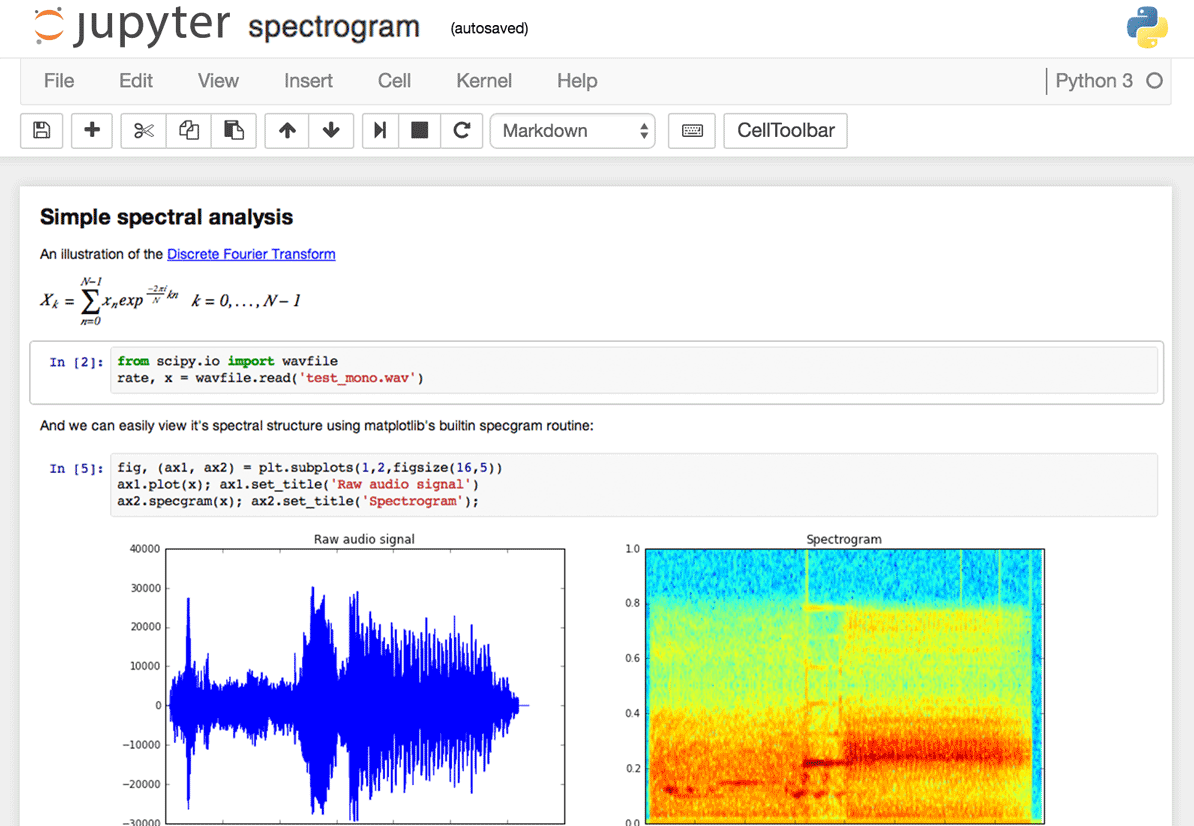
\includegraphics[width=0.98\textwidth]{Bilder/jupyter.png}}
    \caption[Jupyter Notebook]{Beispielhafte Abbildung eines Jupyter Notebooks mit Python-Code und Beschreibung in Textform}
    \label{fig:Bild3.5}
\end{figure}